\section{Proximal Policy Optimization (PPO)}
\begin{frame}{}
    \LARGE Policy Search: \textbf{Proximal Policy Optimization (PPO)}
\end{frame}

\begin{frame}{Proximal Policy Optimization (PPO)}
\begin{itemize}
    \item PPO is motivated by the same question as TRPO: how can we take the biggest possible improvement step on a policy using the data we currently have, without stepping so far that we accidentally cause performance collapse?
    \item Where TRPO tries to solve this problem with a complex second-order method, PPO is a family of first-order methods that use a few other tricks to keep new policies close to old. 
    \item It approximately enforce KL constraint without computing natural gradients.
    \item PPO methods are significantly simpler to implement, and empirically seem to perform at least as well as TRPO.
    \item There are two primary variants of PPO: PPO-Penalty and PPO-Clip.
    
\end{itemize}
\footnotetext{https://spinningup.openai.com/en/latest/algorithms/ppo.html}
    
\end{frame}

\begin{frame}{Proximal Policy Optimization (PPO)}
\begin{itemize}
    \item Adaptive KL Penalty
    \begin{itemize}
        \item Policy update solves unconstrained optimization problem
        $$\theta{k+1} = \arg \max_\theta \mathcal{L}_{\theta_k}(\theta) - \beta_k \overline{D}_{KL}(\theta||\theta_k)$$
        \item Penalty coefficient $\beta_k$ changes between iterations to approximately enforce KL-divergence constraint
    \end{itemize}
    \pause
    \item Clipped Objective
    \begin{itemize}
        \item New objective function: let $r_t(\theta) = \frac{\pi_{\theta}(a_t | s_t)}{\pi_{\theta_k}(a_t | s_t)}$. Then,
        $$\mathcal{L}^{CLIP}_{\theta_k} = E_{\tau \sim \pi_k} \left [ \sum^{T}_{t=0} \left [ r_t(\theta)\hat{A}^{\pi_k}_t, clip(r_t(\theta), 1-\epsilon, 1+\epsilon)\hat{A}^{\pi_k}_t \right ] \right ]$$
        \item $\epsilon$ is a hyperparameter (e.g., $\epsilon = 0.2$)
        \item Policy update is 
        $$\theta_{k+1} = \arg \max_\theta \mathcal{L}^{CLIP}_{\theta_k}$$
        
    \end{itemize}

    
\end{itemize}
    
\end{frame}

\begin{frame}{Proximal Policy Optimization (PPO)}
\begin{figure}
\centering
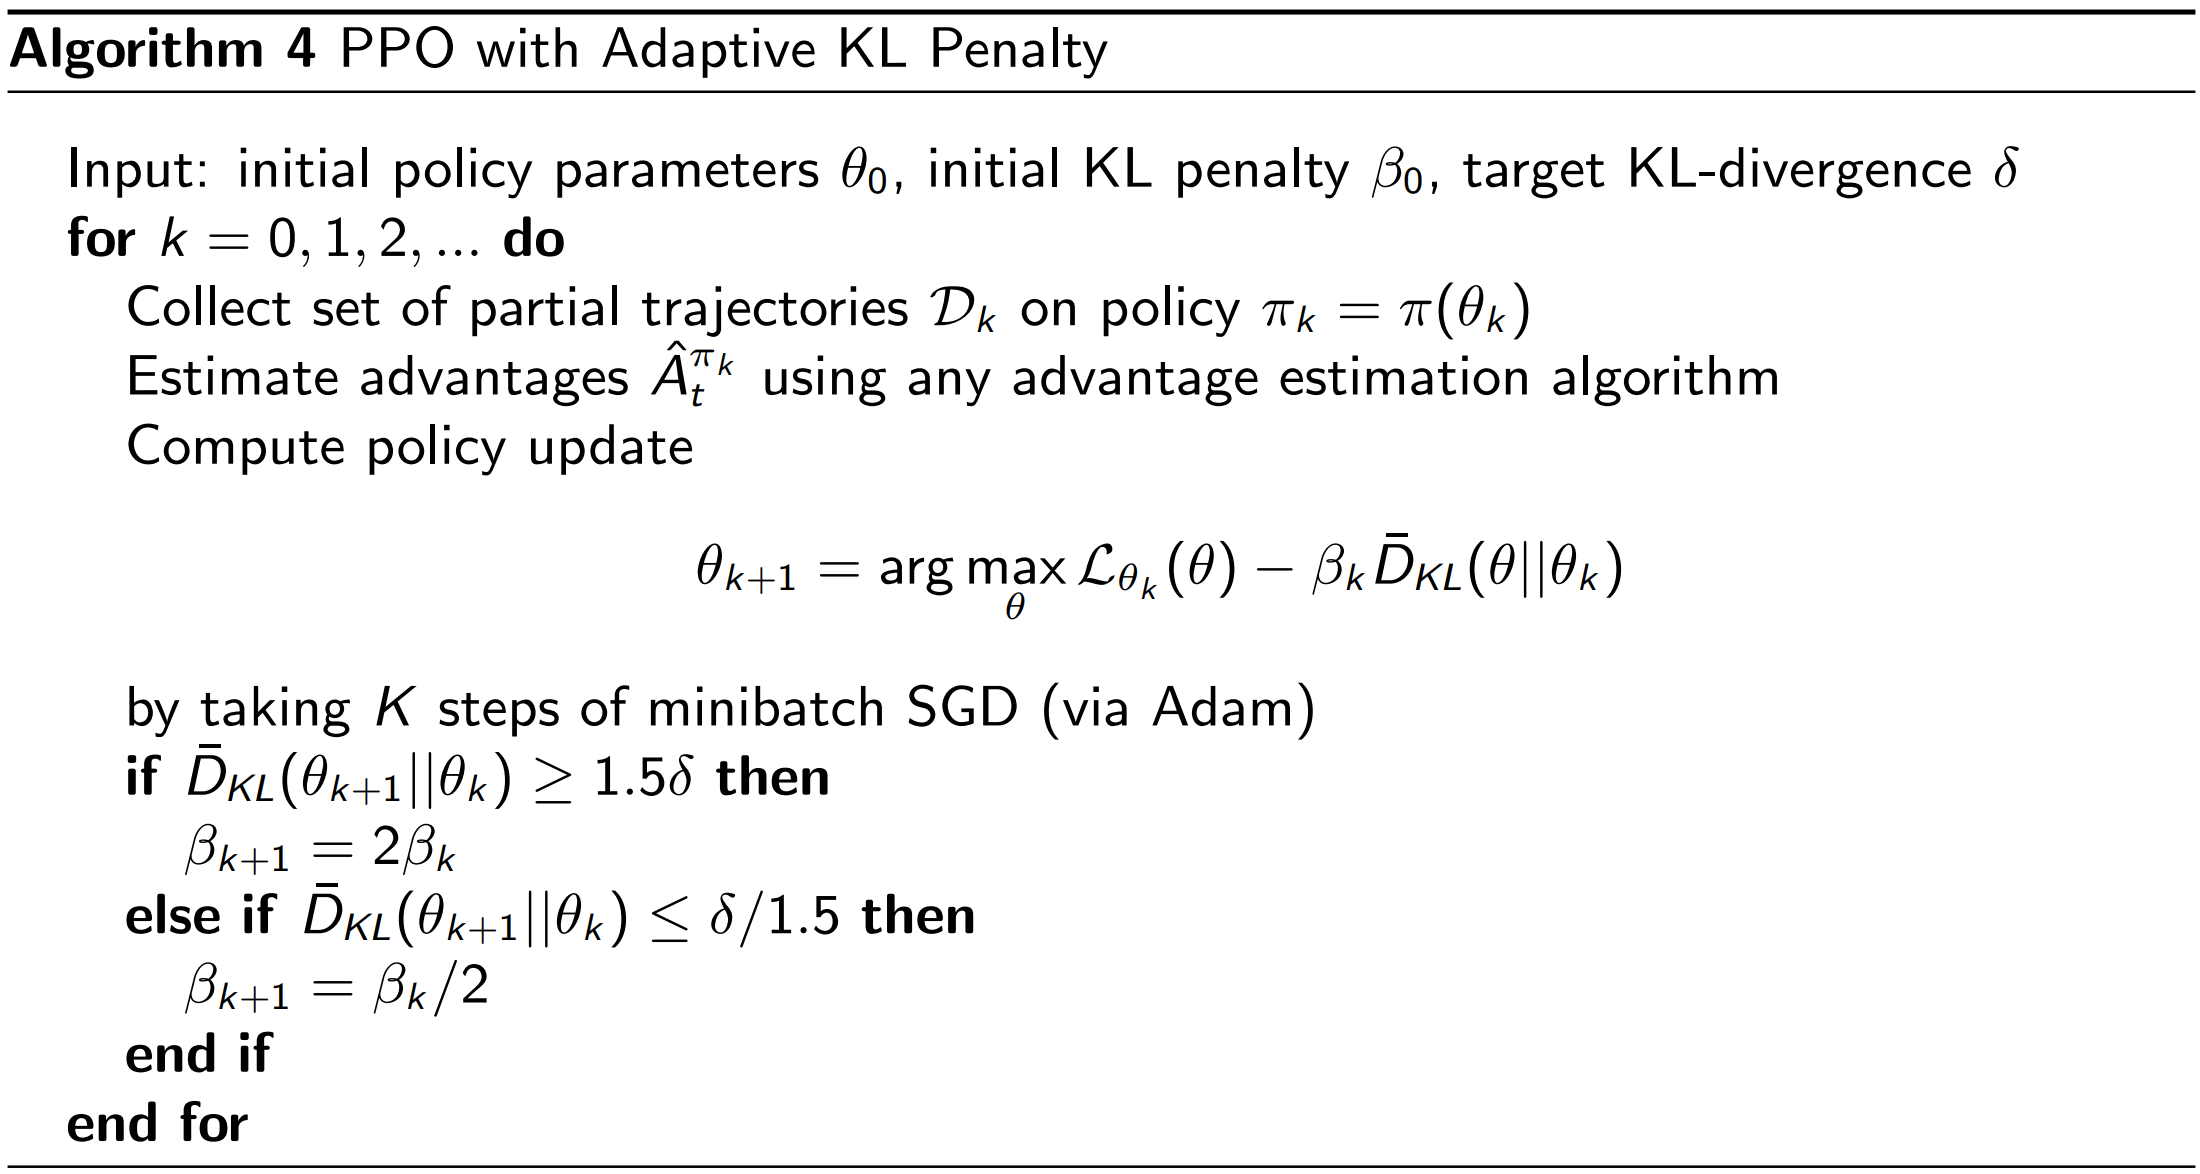
\includegraphics[width=0.9\textwidth,height=0.9\textheight,keepaspectratio]{images/policy-search/ppo_1.png}
\end{figure}
    
\end{frame}

\begin{frame}{Proximal Policy Optimization (PPO)}
\begin{itemize}
    \item PPO clip is more widely used as it seems to work at least as well as PPO with KL penalty, but is simpler to implement
\end{itemize}
\begin{figure}
\centering
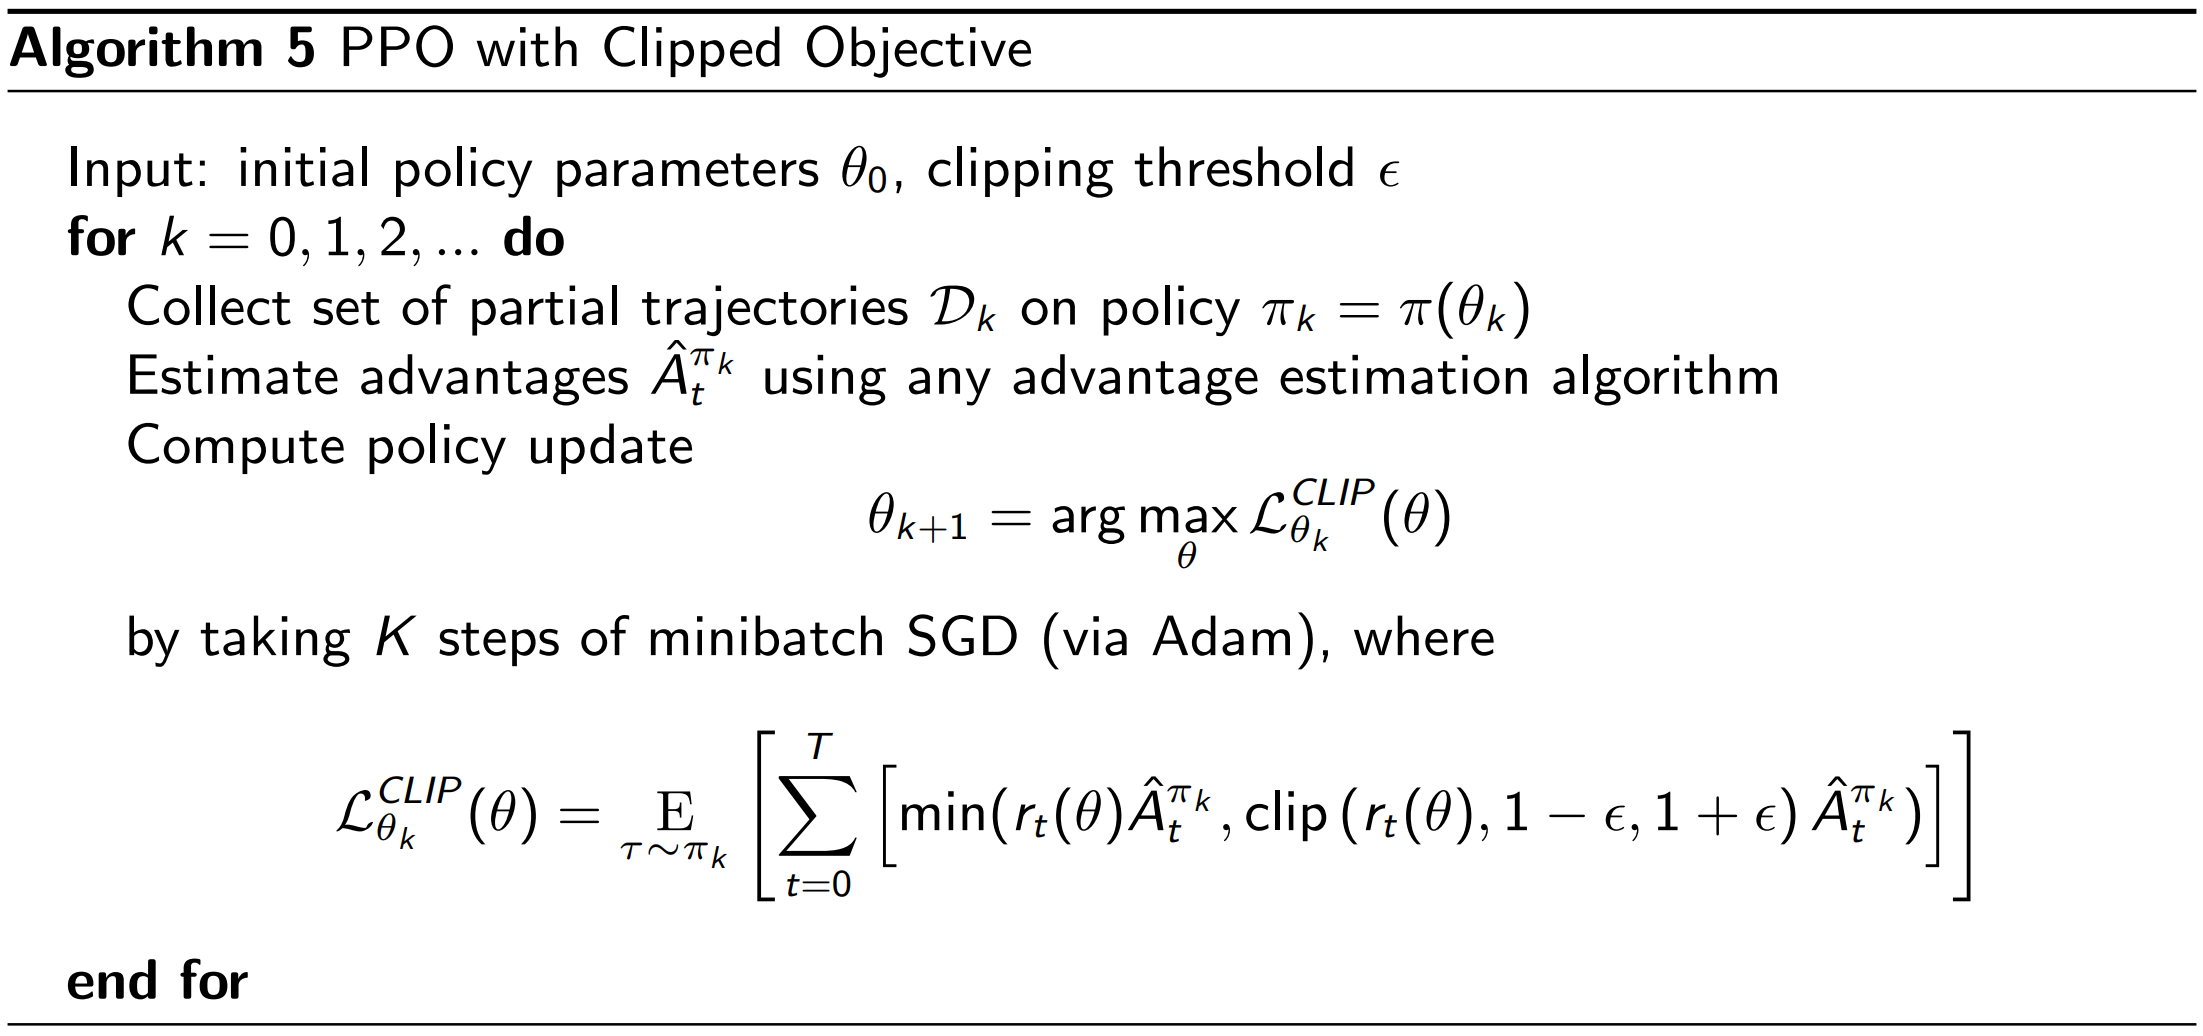
\includegraphics[width=0.9\textwidth,height=0.8\textheight,keepaspectratio]{images/policy-search/ppo_2.png}
\end{figure}
    
\end{frame}

\begin{frame}{Empircal Performance of PPO}
\begin{figure}
\centering
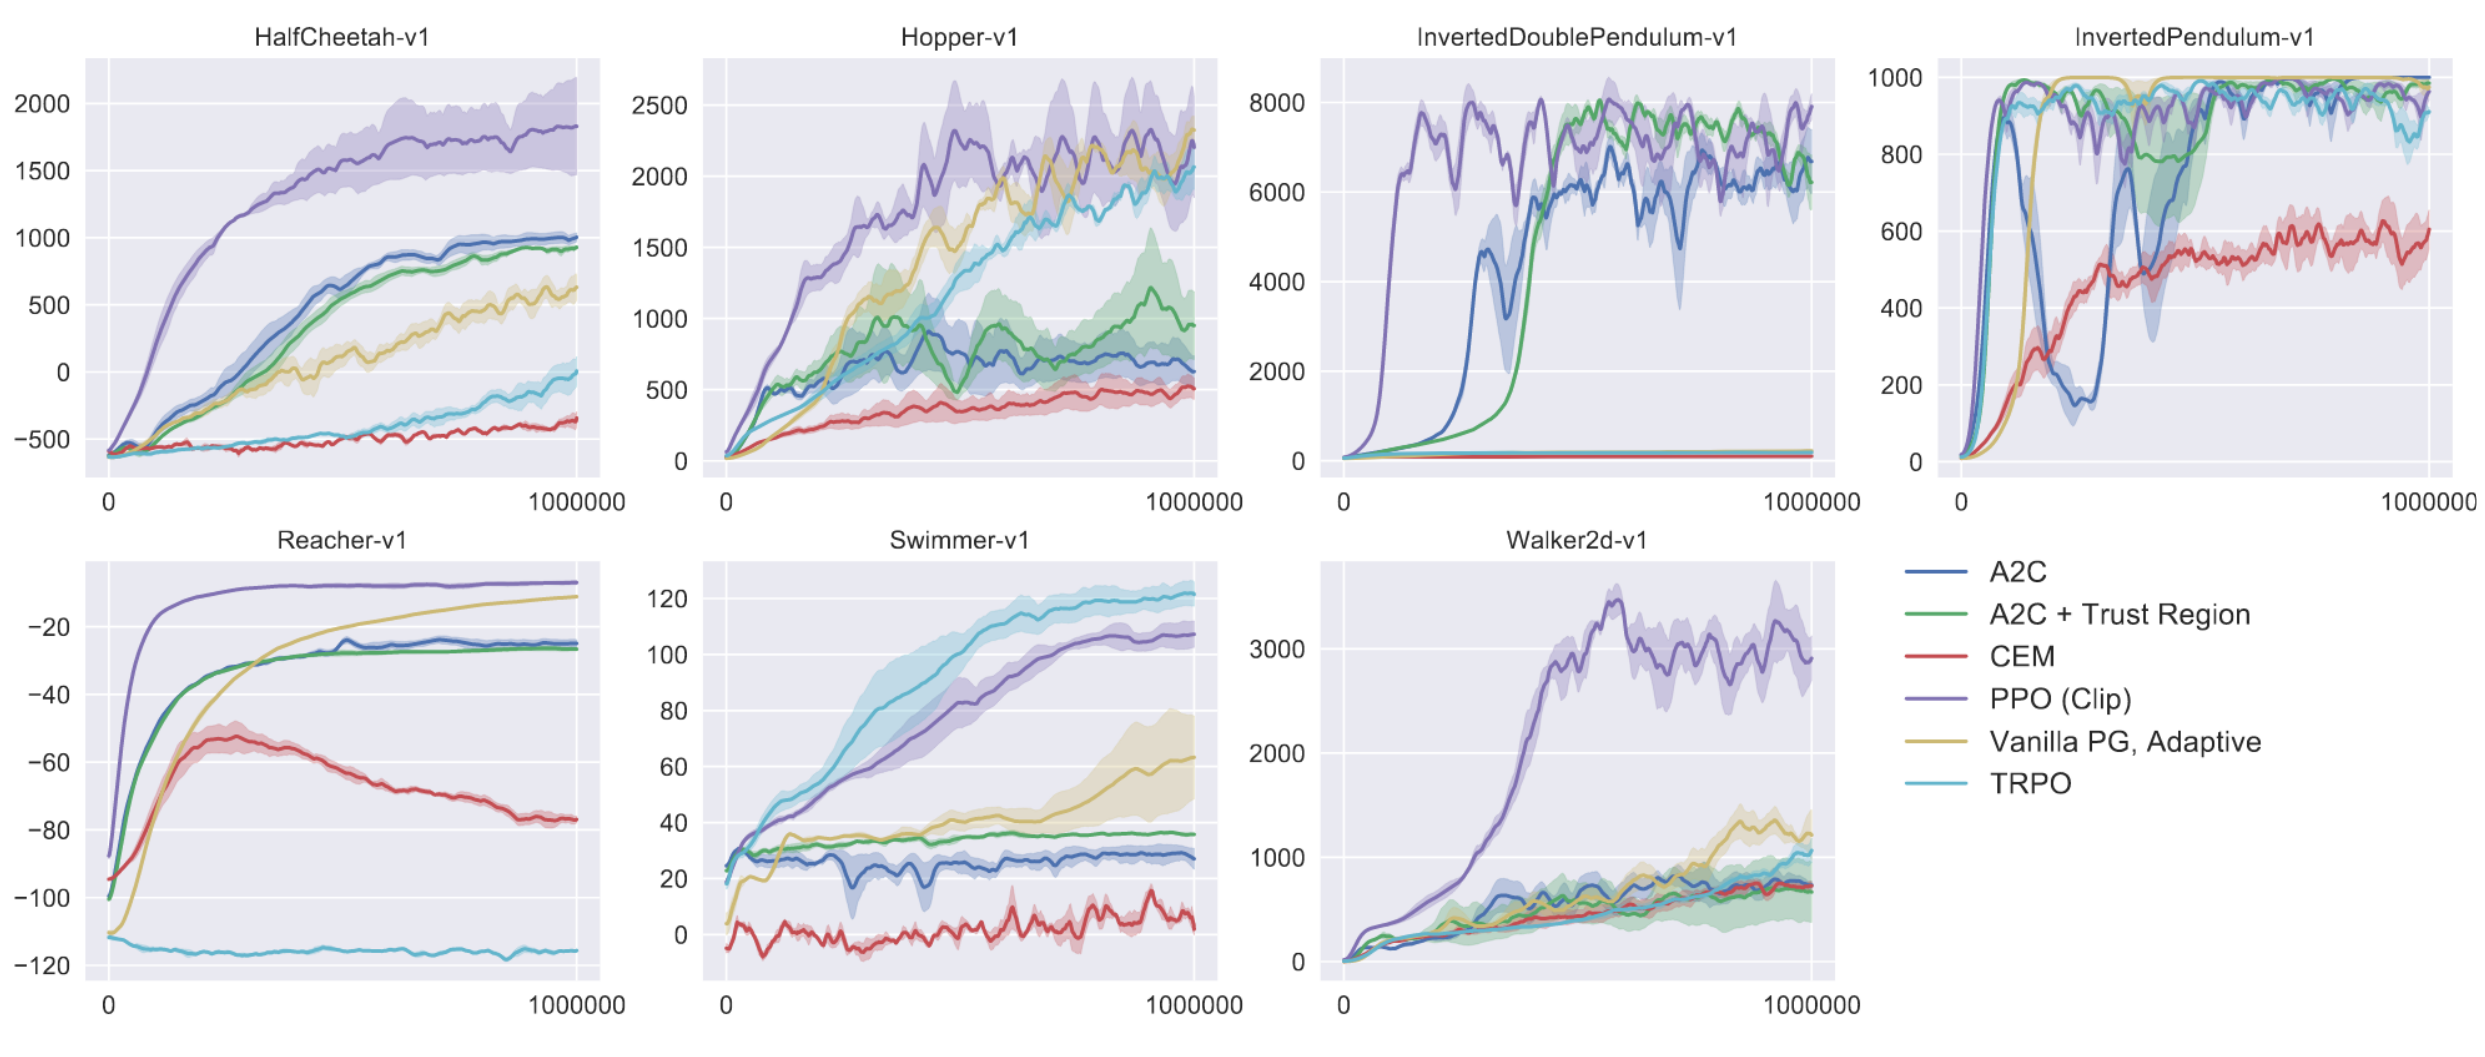
\includegraphics[width=1.0\textwidth,height=1.0\textheight,keepaspectratio]{images/policy-search/ppo_3.png}
\end{figure}

\footnotetext{Schulman, Wolski, Dhariwal, Radford, Klimov, 2017}

\end{frame}